\documentclass{article}[12pt]
\usepackage[a4paper, margin=1in]{geometry}
\usepackage[utf8]{inputenc}
\usepackage[english]{babel}
\usepackage{amssymb, amsmath, amsthm} % math symbols
\usepackage{hyperref} % hyperlinks
\usepackage[table]{xcolor} % tables
\usepackage{graphicx}

\hypersetup{
    colorlinks=true,
    linkcolor=black,
    citecolor=black,
    urlcolor=blue,
    pdfborderstyle={/S/U/W 1}
    }

% title
\title{Learning Notation: Seminar Two \\ Set Theory}
\author{Jack (Quan Cheng) Xie}
\date{}
    
% paragraph /indent spacing
\setlength{\parskip}{6pt}
\setlength{\parindent}{0pt}

% mathtools equation numbering
\counterwithin*{equation}{section}
\renewcommand\theequation{\thesection.\arabic{equation}}

% amsthm theorems formatting
\newtheorem{theorem}{Theorem}

\newtheorem{conjecture}{Conjecture}

\newtheorem{proposition}{Proposition}

\newtheorem{definition}{Definition}

\newtheorem{paradox}{Paradox}

\newtheorem{exercise}{Exercise}

% special symobls
\newcommand{\N}{\mathbb{N}}
\newcommand{\Z}{\mathbb{Z}}
\newcommand{\Q}{\mathbb{Q}}
\newcommand{\R}{\mathbb{R}}
\newcommand{\C}{\mathbb{C}}
\newcommand{\PS}{\mathcal{P}}

% text box for definitions and theorems
\newcommand{\textbox}[1]{\fbox{\parbox{\textwidth}{#1}}}

% bibliography formatting
\makeatletter
\renewcommand{\@biblabel}[1]{$\triangleright$}
\makeatother

\begin{document}

    \maketitle
        
    \section{Sets and Membership}
    
    \subsection{Elements and membership}
        
        \textbox{
        \begin{definition}[Naive set]
            \label{def:inf-function}
                A \textbf{set} is an unordered collection of unique objects. The objects in a set are called its \textbf{elements.}
        \end{definition}
        }
        
        For example, if some unique variables $a, b, c$ are the elements of the set $S$, we can write
        \begin{equation}
            S = \{a, b, c\}. \label{abc-set}
        \end{equation}
        Then $a, b, c$ are elements of $S$, which we can express as
        \begin{equation}
            a, b, c \in S. \label{abc-elements}
        \end{equation}
        The ``$\in$" symbol is read ``is an element of" or ``are elements of." We can also say that $a, b, c$ are \textbf{members} of $S$, $a, b, c$ \textbf{belong} to $S$, and $S$ \textbf{contains} $a, b,$ and $c$.
        If $S = \{a, b, c\}$, then for some other unique element $d$ not in the set, we can write
        \begin{equation}
            d \notin S = \{a, b, c\}.
        \end{equation}
        The elements of a set must be \textbf{unique}, meaning a set cannot contain more than one of the same thing. For example, it would be slightly improper to write
        \begin{equation}
            S = \{a, a, b, c\},
        \end{equation}
        since the element $a$ is not unique in $S$. Alternatively, we can say that
        \begin{equation}
            \{a, a, b, c\} = \{a, b, c\},
        \end{equation}
        by ignoring the repeated element $a$.
    
        \begin{exercise}
            For a set $A$, does $a_1, a_2, a_3 \in A$ imply $A = \{a_1, a_2, a_3\}?$
        \end{exercise}
        
        
    \subsection{Set equality and element order}
        
        Two sets are \textbf{equal} if they have the same elements, regardless of the order of the elements. For example,
        \begin{equation}
            \{a, b, c\} = \{c, b, a\}.
        \end{equation}
        
    \subsection{Cardinality}
        
        A set is \textbf{infinite} if it has infinitely many members. Otherwise it is \textbf{finite.} For example, the set
        \begin{equation}
            \N = \{0, 1, 2, 3, ...\}, \label{naturals}
        \end{equation}
        containing all natural numbers (non-negative integers) is infinite.
        
        The \textbf{cardinality} or \textbf{size} of a set is the number of elements it has. For a set $S$, we write its cardinality as $|S|.$ For example, if $S = \{a, b, c\}$ then
        \begin{equation}
            |S| = |\{a, b, c\}| = 3.
        \end{equation}
        
        Two sets are \textbf{equicardinal} if they have the same cardinality. For example, if
        \begin{align}
            A = \{1, 2, 3, 4, 5\}, \quad B = \{3, 4, 5, 6, 7\},
        \end{align}
        then $|A| = |B| = 5$, so $A$ and $B$ are equicardinal. This is a very informal definition of cardinality. We will look at a more formal definition of equicardinality when discussing functions.
        
    \subsection{Empty set, sets as elements}
    
        The \textbf{empty set} is a special set that contains no elements. We denote it by $\varnothing$ or $\{\}$. A set can have other sets as its members. For example, the following are valid sets:
        \begin{align}
            A &= \{a, b, c\}, \quad B = \{1, 2, 3\},
            \\
            C &= \{\varnothing, A, B\} = \{\{\}, \{a, b, c\}, \{1, 2, 3\}\},
            \\
            D &= \{\varnothing, a, b, c, 1, 2, 3, C\}
            = \{\{\}, a, b, c, 1, 2, 3, \{\{\}, \{a, b, c\}, \{1, 2, 3\}\}\}.
        \end{align}
        
        \begin{exercise}
            What are $|D|$, $|\varnothing|$, and $|\{\varnothing\}|$?
        \end{exercise}
    
    \subsection{Number systems}
        
        We've seen the empty set $\varnothing$, which is a special concept in set theory. Now we will look at some other commonly used sets and their conventional notation.
        
        The set of all \textbf{natural numbers}, which has only positive whole number elements (and zero), is denoted as
        \begin{equation}
            \N = \{0, 1, 2, 3, ...\}.
        \end{equation}
    
        The set of all \textbf{integers}, which contains all positive and negative whole numbers and zero, is denoted as
        \begin{equation}
            \Z = \{0, 1, -1, 2, -2, 3, -3, 4, -4...\}.
        \end{equation}
        
        The set of all \textbf{rational numbers}, which contains all integers that can be written as a fraction of integers, is denoted as
        \begin{equation}
            \Q
            = \left\{...,
            -\frac{2}{3}, -\frac{1}{4}, -\frac{3}{1}, -\frac{1}{3}, -\frac{2}{1}, -\frac{1}{2}, -\frac{1}{1},\ 
            \frac{0}{1},\
            \frac{1}{1},\ \frac{1}{2},\ \frac{2}{1},\ \frac{1}{3}, \frac{3}{1},\ \frac{1}{4},\ \frac{2}{3},
            ...\right\}
        \end{equation}
        
        The set of all \textbf{real numbers} is written as
        \begin{align}
            \R
            &= (-\infty, \infty), \label{reals-interval}
        \end{align}
        which contains numbers like $\pi, e,$ and $\sqrt{2}$ that cannot be expressed as fractions of integers.
        
        % \textbox{
        % \begin{proposition}
        %     The number $\sqrt{2}$ is irrational.
        % \end{proposition}
        % }
        % \begin{proof}
        %     By contradiction, suppose that $\sqrt{2}$ is rational. Then there exists $p, q \in \Z$ with no common factors where $\sqrt{2} = \frac{p}{q}$. Then we have that
        %     \begin{align*}
        %         \sqrt{2} = \frac{p}{q}
        %         & \implies
        %         2 = \frac{p^2}{q^2} \\
        %         & \implies
        %         p^2 = 2 p^2.
        %     \end{align*}
        %     Since $p$ is an integer, then $p$ must be divisible by 2, thus $p = 2m$ for some $m \in \Z$. Then we have that \begin{align*}
        %         2 q^2 = p^2, p = 2m
        %         & \implies
        %         2 q^2 = 4m^2 \\
        %         & \implies 
        %         q^2 = 2m^2.
        %     \end{align*}
        %     Since $q$ is also an integer, it must also be divisible by 2. Then both $p$ and $q$ are divisible by two, which contradicts the statement that they have no common factors.
        % \end{proof}
        
        We also have the set of complex numbers, denoted by $\C$, which can be constructed from all pairs of real numbers $x, y \in \R$. We have $x$ for the real component, and add it to $y$ times $i = 
        \sqrt{-1}$, the imaginary component. We can write the complex numbers using set builder notation:
        \begin{align}
            \C
            &= \left\{ x + y i \; : \; x, y \in \R, \; i = \sqrt{-1} \label{complex} \right\}
        \end{align}
        
        % \begin{exercise}
        %     Show that $\sqrt{3}$ is irrational.
        % \end{exercise}
        
    \subsection{Set builder notation}
        
        Up to now we have mostly been explicitly writing sets with \textbf{set roster notation}. The can be a little vague if we are not careful. Instead we can use \textbf{set builder notation} to precisely specify what elements we want in a defined set. Set notation specifies the elements of the set by using predicates:
        \begin{align}
            x \in X \land P(x) \iff x \in \{y \in X : P(y)\}.
        \end{align}
        For example, we can write the set of all positive real numbers $\R$ as
        \begin{equation}
            (0, \infty) = \{x \in \R : x > 0\}. \label{R-plus}
        \end{equation}
        
        We sometimes call this set $\R^+$. The ``$:$" symbol can be read \textbf{``where"} or \textbf{``such that."} Sometimes we use ``$|$" instead of ``$:$". The right hand side of \eqref{R-plus} is read, "the set of all elements $x$ in the reals where $x$ is greater than zero."
        
        \begin{exercise}
            Construct $\Z$ and $\Q$ from $\N$ with set builder notation.
        \end{exercise}
        
    \subsection{Tuples and Cartesian product}
        
        \textbox{
        \begin{definition}[Tuple]
            Informally, a \textbf{tuple} is a finite, ordered list (or sequence) of elements. A \textbf{n-tuple} is a tuple of $n$ elements.
            \begin{align}
                (a_1, a_2, a_3, ..., a_n).
            \end{align}
        \end{definition}
        
        \begin{definition}[Cartesian product]
            The \textbf{Cartesian product} of two sets $A$ and $B$ is the set of all pairs (or 2-tuples) of elements $(a, b)$ from $a \in A$ and $b \in B$.
            \begin{align}
                C = A \times B = \{(a, b) : a \in A, b \in B\}
            \end{align}
            
            We can generalize to the definition of a $n$-ary Cartesian product of arbitrary many sets:
            \begin{align}
                X_1 \times ... \times X_n
                = \{(x_1, ..., x_n) : x_i \in X_i, \forall i \in \{i, ..., n\}\}
            \end{align}
        \end{definition}
        }
            
    \subsection{Russell's paradox}
    
        So far we have allowed pretty much anything to be a member of a set, including other sets. However, if we are not careful with our formulation of what sets are, we can run into some bizarre problems. The logician Bertrand Russell came up with a famous paradox that arises from a naive definition of a set.
        
        \textbox{
        \begin{paradox}[Russell]
            Let $R$ be the set of all sets which are not members of themselves.
            \begin{align}
                R = \{S : S \not\in S\}.
            \end{align}
            Then we have that $R$ is a member of itself if and only if it is not a member of itself.
            \begin{align}
                R \in R \iff R \not\in R.
                \label{eqn:russell}
            \end{align}
        \end{paradox}
        }
        
        The definition of $R$ states for any set $S$ in the universe of all sets, we have $S \notin S \implies S \in R$. Since $R$ is also a set, if we let $S = R$, then $R \notin R \implies R \in R$, which is the converse in \eqref{eqn:russell}.
        
        The (logically equivalent) contrapositive of the definition is that for any sets $S$, $S \in R \implies S \not\in R$. Then letting $S = R$ means $R \in R \implies R \not\in R,$ the conditional statement in \eqref{eqn:russell}.
        
        Then both the implication $R \notin R \implies R \in R$ and converse $R \in R \implies R \not\in R$ are true, which means the biconditional statement $R \notin R \iff R \in R$ is true. But this biconditional statement is a contradiction, which is always false.
        
        Together this shows that the set $R$ which contains all sets other except itself can neither contain itself or not contain itself---a paradox.
    
        To resolve such paradoxes, mathematicians limit what are allowed to be valid sets, which is standardized with the \href{https://en.wikipedia.org/wiki/Zermelo\%E2\%80\%93Fraenkel_set_theory}{Zermelo-Fraenkel axioms} (ZF axioms). However, problems with naive set theory apparently rarely come up unless you specifically look for them (like in the case of Russell's paradox), so we will not worry about it.
        
        
    \section{Set Operations and Subsets}
    
    \subsection{Union}
    
        \textbox{
        \begin{definition}[Union]
            The \textbf{union} of sets $A$ and $B$ are defined as
            \begin{align}
                A \cup B = \{ x : (x \in A) \lor (x \in B) \}.
            \end{align}
        \end{definition}
        }
        
        For example, if $A = \{a, b, c\}$ and $B = \{b, c, d, e\}$ then $A \cup B = \{a, b, c, d, e\}$.
            
    \subsection{Intersection}
        
        \textbox{
        \begin{definition}[Intersection]
            The \textbf{intersection} of sets $A$ and $B$ are defined as
            \begin{align}
                A \cap B = \{ x : (x \in A) \land (x \in B) \}.
            \end{align}
        \end{definition}
        }
        
        For example, if $A = \{a, b, c\}$ and $B = \{b, c, d, e\}$ then $A \cap B = \{b, c\}$.
    
    \subsection{Difference and complement}
        \textbox{
        \begin{definition}[Set difference]
            The \textbf{difference} between sets $A$ and $B$ are defined as
            \begin{align}
                A \setminus B = \{ x : (x \in A) \land (x \not\in B) \}.
            \end{align}
        \end{definition}
        }
        
        For example, if $A = \{a, b, c\}$ and $B = \{b, c, d, e\}$, then $A \setminus B = \{a\}$ and $B \setminus A = \{d, e\}$.
        
    \subsection{Subset and superset}
    
        \textbox{
        \begin{definition}[Subset and superset]
            $A$ is a \textbf{subset} of $S$ if and only if
            \begin{equation}
                A \cap S = A.
            \end{equation}
            Then we write that $A \subseteq S$. We also call $S$ the \textbf{superset} of $A$ and write $S \supseteq A$.
        \end{definition}
    
        \begin{definition}[Proper subset and superset]
            $A$ is a \textbf{proper subset} of $S$ if and only if
            \begin{equation}
                A \subseteq S
                \quad\text{and}\quad
                (S \setminus A) \ne \varnothing.
            \end{equation}
            Then we write $A \subset S$. We also call $S$ the \textbf{proper superset} of $A$ and write $S \supset A$.
        \end{definition}
        }
            
        \textbox{
        \begin{definition}[Complement]
            Given a \textbf{universal set} $U$ which is a superset of $A$, we define the \textbf{complement} of set $A$ as
            \begin{align}
                A^c = \bar A = U \setminus A
            \end{align}
        \end{definition}
        }
        
        \textbox{
        \begin{theorem}[De Morgan's laws]
            \begin{align}
                A \cup B &= (A^c \cap B^c)^c,
                \label{thm:de-morgan1}
                \\
                A \cap B &= (A^c \cup B^c)^c.
                \label{thm:de-morgan2}
            \end{align}
        \end{theorem}
        }
        \begin{proof}
            For any element $x$, if $p := x \in A$ and $q := x \in B$, then
            \begin{align}
                x \in A \cup B
                &\iff (x \in A) \lor (x \in B)
                \iff p \lor q,
            \\
                x \in A \cap B
                &\iff (x \in A) \land (x \in B)
                \iff p \land q,
            \end{align}
        
        For complements we can show that $r = y \in S \implies \neg r = y \in S^c$:
            \begin{align}
                r = y \in S
                \implies y \in S^c
                &\iff 
                y \not\in S \text{ or } \neg (y \in S)
                \iff \neg r.
            \end{align}
            
        Then write \eqref{thm:de-morgan1} and \eqref{thm:de-morgan2} as
            \begin{align}
                A \cup B &= (A^c \cap B^c)^c 
                \iff p \lor q \equiv \neg(\neg p \land \neg q),
                \\
                A \cap B &= (A^c \cup B^c)^c
                \iff p \land q \equiv \neg(\neg p \lor \neg q),
            \end{align}
            which we've previously proved with truth tables.
        \end{proof}
        
        
    \subsection{Power set}
        
        \textbox{
        \begin{definition}[Power set]
            The \textbf{power set} of $S$, denoted $\PS(S)$ or $2^S$, is the set of all subsets of $S$:
            \begin{align}
                \PS(S) = \{A : A \subseteq S\}.
            \end{align}
        \end{definition}
        }
        
        For example, $\PS(\{a, b\}) = \{\varnothing, \{a\}, \{b\}, \{a, b\}\}$.
        
        \begin{exercise}
            What is $\PS(\varnothing)$? What is $\PS(\PS(\varnothing))$ and $\PS(\PS(\PS(\varnothing)))$?
        \end{exercise}
        
        \begin{exercise}
            Prove by induction that $|\PS(S)| = 2^{|S|}$ for any finite set $S$.
        \end{exercise}
    
    \section{Functions}
        
        We can define functions in relation to sets.
                
        \textbox{
        \begin{definition}[Function]
        \label{def:function}
            A \textbf{function} from a set $X$ to $Y$ maps each element in $X$ to exactly one element in $Y$. We denote the function as $f : X \to Y$. \\
            
            $X$ is called the \textbf{domain} of the function and $Y$ is called its \textbf{co-domain}.
        \end{definition}
        }
        
        We can also write explicity. For example, $f(x) = \ln x$ and $x \mapsto \ln x$, which are two ways to write the same function.
    
    
    \subsection{Image}
    
        \textbox{
        \begin{definition}[Image]
            For a function $f : X \to Y$, the \textbf{image} of a subset of the domain $A \subseteq X$ are the set of $f(a)$ for every $a \in A$:
            \begin{align}
                f(A) = \{f(a) : a \in A\}.
            \end{align}
        \end{definition}
        
        \begin{definition}[Range]
            For a function $f : X \to Y$, the \textbf{range} of the function is the image of the domain:
            \begin{align}
                f(X) = R = \{f(x) : x \in X\}.
            \end{align}
        \end{definition}
        }
        
        \textbox{
        \begin{definition}[Preimage]
            For an element $y$ in the co-domain $Y$, the set of elements in the domain $X$ hat maps to $y$ is the \textbf{preimage} of $y$:
            \begin{align}
                f^{-1}(y) = \{x : f(x) = y\}.
            \end{align}
            
            We similarly define the preimage of a subset of the co-domain $B \subseteq Y$ as:
            \begin{align}
                f^{-1}(B) = \{x : f(x) \in B\}.
            \end{align}
        \end{definition}
        }
        
        For example, for the real function $f(x) = x^2$, the preimage $f^{-1}(4) = \{2, -2\}$, and $f^{-1}(\{1, 4\}) = \{-2, -1, 1, 2\}$. What is $f^{-1}(\{n^2 : n \in \N\})$?
        
    \subsection{Injection, surjection, and bijection}
        
        \textbox{
        \begin{definition}[Injection]
            An \textbf{injective function} (or \textbf{injection}, or \textbf{one-to-one function}) is a function where each element in the co-domain is assigned at most once.
            \begin{align}
                \forall x, x' \in X, \;
                f(x) = f(x') \implies x = x'.
            \end{align}
        \end{definition}
        }
        
        \textbox{
        \begin{definition}[Surjection]
            An \textbf{surjective function} (or \textbf{surjection}) is a function where each element in the co-domain is assigned at least once.
            \begin{align}
                \forall y \in Y,\;
                \exists x\in X ,\; 
                y = f(x).
            \end{align}
        \end{definition}
        }
        
        \textbox{
        \begin{definition}[Bijection]
            A \textbf{bijective function} (or \textbf{bijection}, or \textbf{one-to-one correspondence}, or \textbf{invertible function}) is a function that is both an injection and a surjection.
            \begin{align}
                \forall y \in Y,\;
                \exists! x\in X ,\; 
                y = f(x),
            \end{align}
            where $\exists! x$ means there exists exactly one $x$.
        \end{definition}
        }
        
        See Figure \ref{fig:functions} for illustrations.
        
        \begin{figure}[!ht]
            \centering
            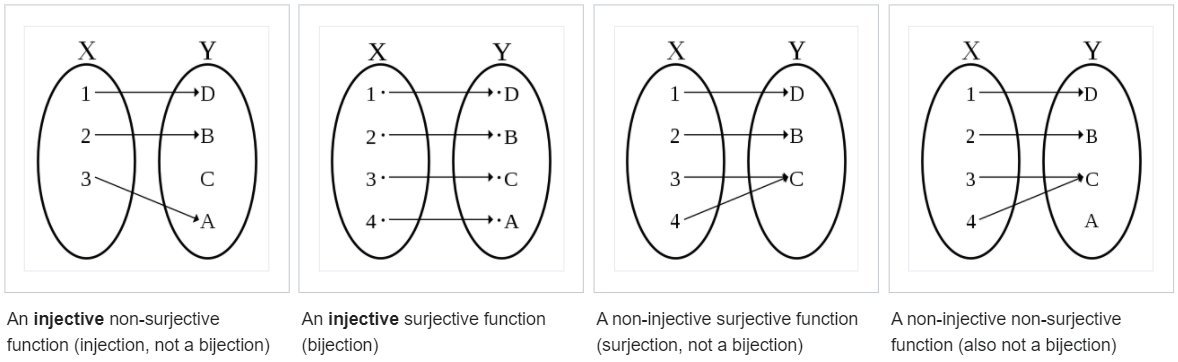
\includegraphics[width=\textwidth]{attachments/2.1-functions.png}
            \caption{Illustrations of functions from \href{https://en.wikipedia.org/wiki/Bijection}{Wikipedia}}
            \label{fig:functions}
        \end{figure}
    
    \subsection{Equicardinality}
        
        \textbox{
        \begin{definition}[Equicardinality]
            Two sets are \textbf{equicardinal} if there exists a bijective function between them.
        \end{definition}
            }
            
        \begin{exercise}
            Are set of all natural numbers $\N$ and the set of all even numbers equicardinal? What about the naturals and odd numbers? How can you prove it?
        \end{exercise}
    
    
    \section{Countability and infinite sets}
    
    \subsection{Countable sets}
    
        \textbox{
        \begin{definition}
            A set is \textbf{countable} if it is either finite or equicardinal to $\N$. Otherwise, it is \textbf{uncountable.}
        \end{definition}
        }
        
        We call the cardinality of countably infinite sets $\aleph_0$ (``aleph null"). Both $\Z$ and $\Q$ are countable as they are equicardinal to $\N$.
        
        To show that the integers is countable, we can arrange the its elements in alternating order of negative and positive naturals:
        \begin{align}
            \Z
            = \{0, 1, -1, 2, -2, ...\}
            = \{z_0, z_1, z_2, z_3, z_4, ...\}.
        \end{align}
        
        Since this arrangement ensures all integers are captured by the pattern, we can assign a natural number to each integer with indexing.
        
        For the rationals, we can also arrange them in an exhaustive, indexable list. We can list all the non-negative rationals by grouping fractions where the numerator and denominator sum to be the same.
        \begin{align}
            \Q_{\ge 0} = \left\{\frac{0}{1}, \frac{1}{1}, \frac{1}{2}, \frac{2}{1}, \frac{1}{3}, \left(\frac{2}{2},\right) \frac{3}{1}, \frac{1}{4}, \frac{2}{3}, \frac{3}{2}, ... \right\}
            = \left\{0, 1, \frac{1}{2}, 2, \frac{1}{3}, 3, \frac{1}{4}, \frac{2}{3}, \frac{3}{2}, ... \right\}
        \end{align}
        Then we can include the negative rationals in the list by inserting them after their positive counterpart, just as in the integers, and index the list.
        \begin{align}
            \Q
            &= \left\{0,
            \ 1, -1,
            \ \frac{1}{2}, -\frac{1}{2},
            \ 2, -2,
            \ \frac{1}{3}, -\frac{1}{3},
            \ 3, -3,
            % \ \frac{1}{4}, -\frac{1}{4},
            % \ \frac{2}{3}, -\frac{2}{3},
            % \ \frac{3}{2}, -\frac{3}{2},
            ... \right\}
            = \bigg\{q_0,
            \ q_1,\ q_2,
            \ q_3,\ q_4,
            \ q_5,\ q_6,
            ... \bigg\}
        \end{align}
    
        More generally, an infinite set is ``listable" if (and only if) it is countable.
        
        Other countable sets include those of all
        \begin{itemize}
            \item
            constructible numbers
            
            \item
            computable numbers: set of reals computable to arbitrary precision
            
            \item
            algebraic numbers: root solutions to polynomials
            
            \item
            finite strings of zeros and ones
            
        \end{itemize}
            
        
        
    \subsection{Uncountable sets}
    
        \href{https://www.youtube.com/watch?v=elvOZm0d4H0}{Georg Cantor} introduced the concept of countability and produced a famous proof that the set of all real numbers is \textbf{uncountable}.
        
        The cardinality of the reals is called $\aleph_1$ (``aleph one").
        
        Some other sets with this cardinality are:
        
        \begin{itemize}
            \item $\R \setminus \Q$, the difference between the reals and rationals
            
            \item
            The interval $[0, 1]$ (or any non-empty real interval)
            
            \item
            $2^{\N}$, the power set of the natural numbers (or any $\aleph_0$ set)
            
            \item
            $\{0, 1\}^{\infty}$, the set of all infinite-length strings of zeros and ones.
        \end{itemize}
        
        \textbox{
        \begin{theorem}
            The set of real numbers in the interval $[0, 1]$ is uncountable.
        \end{theorem}
        }
        
        \begin{proof}(Contradiction)
            Assume that the real numbers in $[0, 1]$ is countable. Then we should be able to put all of them in a list. Let us represent such list as decimals of infinite-length binary strings, for example like in Table \ref{tab:cantor-diag}.
            
            \begin{table}[!ht]
                \centering
                \begin{tabular}{|r|l|}
                    \hline
                     $n$& 1 2 3 4 5 6 7 8 9 ...
                     \\ \hline\hline
                     0. & \underline{\bf0} 0 0 0 0 0 0 0 0 ...  \\
                     0. & 1 \underline{\bf1} 1 1 1 1 1 1 1 ...  \\
                     0. & 1 0 \underline{\bf0} 0 0 0 0 0 0 ...  \\
                     0. & 1 1 0 \underline{\bf0} 0 0 0 0 0 ...  \\
                     0. & 1 0 1 0 \underline{\bf1} 0 0 0 1 ...  \\
                     0. & 0 1 0 1 1 \underline{\bf1} 0 1 1 ...  \\
                     0. & 0 1 0 0 1 0 \underline{\bf0} 0 1 ...  \\
                     0. & 0 1 0 1 0 0 1 \underline{\bf0} 1 ...  \\
                     \vdots & \hspace{3em} \vdots \\
                     \hline
                \end{tabular}
                \caption{Cantor's Diagonization}
                \label{tab:cantor-diag}
            \end{table}
            
            Then let $a_n$ be the $n$th decimal of the $n$th real number in the countable list, and let
            \begin{align}
                a
                = 0.\ a_1\ a_2\ a_3\ a_4\ a_5\ a_6\ a_7\ a_8\ ...
                = 0.\ 0\ 1\ 0\ 0\ 1\ 1\ 0\ 0\ ...
            \end{align}
            These are the underlined decimals in Table \ref{tab:cantor-diag}. Let $b_n = 1$ if $a_n = 0$, and $b_n = 0$ if $a_n = 1$. Then the string
            \begin{align}
                b
                = 0.\ b_1\ b_2\ b_3\ b_4\ b_5\ b_6\ b_7\ b_8\ ...
                = 0.\ 1\ 0\ 1\ 1\ 0\ 0\ 1\ 1\ ...
            \end{align}
            is a binary real number in $[0, 1]$ that is not included in the list, since each decimal place
            is different from at least one other real number in the list. Thus there can never be a countable list of all real numbers between $[0, 1]$, as one can always construct a new real number not included in the list by this \textbf{diagonlization} method.
        \end{proof}
        
        \begin{exercise}
            Show for any $a, b \in \R$, the cardinality of $[0, 1]$ is equal to that of interval $[a, b]$.
        \end{exercise}
        
        \begin{exercise}
            Show that $\R$ and $\R^+$ are equicardinal.
        \end{exercise}
        
        \begin{exercise}
            See Appendix \eqref{app:interval-cardinalities} for proof that the intervals $[0, 1]$, $[0, 1)$, $(0, 1]$, and $(0, 1)$ are all equicardinal. Show that $[0, 1]$ is equicardinal to $\R$.
        \end{exercise}

    \subsection{Higher cardinalities}
    
        We can show that for any set $A$, its power set has a greater cardinality. This is true even for infinite sets, countable and uncountable.
        
        It is clear that there always exists an injection between a set $A$ and its power-set $\PS(A)$, since $x \mapsto \{x\}$. This means that $|A| \le \PS(A)$.
        
        To prove that $|A| < |\PS(A)|$, we can show that there cannot exist a bijection, that is a function that is both injective and surjective. In particular, there exists no surjection $f: A \to \PS(A)$. This theorem is also due to Georg Cantor.
        
        \textbox{
        \begin{theorem}
            There exists no surjective function $f: A \to \PS(A).$
        \end{theorem}
        }
        
        \begin{proof}(Contradiction)
            Suppose for the sake of contradiction that there exists a surjection $f: A \to \PS(A).$
            
            Then let $B = \{x \in A : x \not\in f(x)\}$, the set of every element in $A$ that is not a member of its own image in the power set. Note that $B \subseteq A$, which means $B \in \PS(A)$.
            
            Since $f : A \to \PS(A)$ is surjective, meaning every member in $\PS(A)$ is mapped to an element in $A$, there must exists some $y \in A$ such that $f(y) = B$.
            
            Then by definition of $B$, we have the following implications:
            \begin{align}
                y &\in f(y) = B \implies y \not\in f(y) = B,
                \\
                y &\not\in f(y) = B \implies y \in f(y) = B.
            \end{align}
            Together this implies that $y \in B \iff y \not\in B$. This is a contradiction, so there must not exist any surjection $f: A \to \PS(A)$.
            
            Since there always exists a injection $h: A \to \PS(A)$, this means that $|\PS(A)| > |A|$.
        \end{proof}
        
        This implies that there are at least countably many cardinalities larger than even $\aleph_1$, each successively larger than the next, since by Cantor's theorem,
        \begin{align*}
            \aleph_1 = | \R |
            &< | \PS(\R) | = \aleph_2,
            \\
            \aleph_2 = | \PS(\R) |
            &< | \PS(\PS(\R)) | = \aleph_3,
            \\
            \aleph_3 = | \PS(\PS(\R)) |
            &< | \PS(\PS(\PS(\R))) | = \aleph_4,
            \\
            &\ \vdots
        \end{align*}
        One famous and important conjecture about infinite cardinalities is the \href{https://www.youtube.com/watch?v=ZC7wglkBWMM}{continuum hypothesis (CH)}.
        
        \textbox{
        \begin{conjecture}[Continuum hypothesis]
            There does not exists a set whose cardinality is strictly between $\aleph_0$ and $\aleph_1$.
        \end{conjecture}
        }
        
        In 1940, Kurt Gödel showed that CH \textbf{cannot be disproven} from Zermelo-Fraenkel set theory with axiom of choice (ZFC). Then in the 1960s, Paul Cohen showed that CH also \textbf{cannot be proven} with ZFC, a result for which he was awarded a Field's Medal.
        
        Gödel also famously showed in his \textbf{incompleteness theorems} that there exists truths in mathematics that cannot be proven.
    
    
    \appendix
    \section{Appendix}
        
        \subsection{Equicardinality of intervals}\label{app:interval-cardinalities}
        
        \textbox{
        \begin{proposition}
            The intervals $(0, 1)$ , $[0, 1)$, $(0, 1]$, and $[0, 1]$ are equicardinal.
        \end{proposition}
        }
        
        \begin{proof}
            We can show there exist bijective functions from $(0, 1)$ to $[0, 1), (0, 1],$ and $[0, 1]$ by \href{https://youtu.be/Uj3_KqkI9Zo}{Hilbert's Hotel} arguments. Let $H = \left\{\frac{1}{n} : n \in \N, n > 1 \right\}$, a countably infinite set which is a proper subset of $\left(0, \frac{1}{2}\right]$.
            
            Define $f_1 : (0, 1) \to [0, 1)$ as
            \begin{align}
                f_1(x) = \begin{cases}
                    0,              & x = \frac{1}{2}
                    \\
                    \frac{1}{n-1},  & x \in \left\{\frac{1}{n} : n \in \N, n > 2\right\}
                    \\
                    x,              & x \not\in H.
                \end{cases}
            \end{align}
            
            Define $f_2 : (0, 1) \to (0, 1]$ as
            \begin{align}
                f_2(x) = \begin{cases}
                    1,              & x = \frac{1}{2}
                    \\
                    \frac{1}{n-1},  & x \in \left\{\frac{1}{n} : n \in \N, n > 2\right\}
                    \\
                    x,              & x \not\in H.
                \end{cases}
            \end{align}
            
            Define $f_3 : (0, 1) \to [0, 1]$ as
            \begin{align}
                f_3(x) = \begin{cases}
                    0,              & x = \frac{1}{2}
                    \\
                    1,              & x = \frac{1}{3}
                    \\
                    \frac{1}{n-2},  & x \in \left\{\frac{1}{n} : n \in \N, n > 3\right\}
                    \\
                    x,              & x \not\in H.
                \end{cases}
            \end{align}
            
        It can be seen that each of these functions is a bijection. Then the open interval is equicardinal to each of the other type of interval, which means they are all equicardinal.
    \end{proof}

    \begin{thebibliography}{9}
        
        \bibitem{stack}
        Ben (https://math.stackexchange.com/users/32139/ben). (2012), \emph{How to define a bijection between $(0,1)$ and $(0,1]$?} math.stackexchange.com. \url{https://math.stackexchange.com/q/160750}
        
        \bibitem{book-of-proof}
        Hammack, Richard, (2018). \emph{Book of Proof, third edition}. Richard Hammack. \url{https://www.people.vcu.edu/~rhammack/BookOfProof/}
        
        \bibitem{iitm-1}
        Jagannathan, Krishna. (2015). \emph{Mod-01 Lec-02 CARDINALITY AND COUNTABILITY-1}, lecture. Probability Foundation for Electrical Engineers. Indian Institute Of Technology–Madras.
        \url{https://youtu.be/gLT58t2z48A}
        
        \bibitem{iitm-2}
        Jagannathan, Krishna. (2015). \emph{Mod-01 Lec-02 CARDINALITY AND COUNTABILITY-2}, lecture. Probability Foundation for Electrical Engineers. Indian Institute Of Technology–Madras.
        \url{https://youtu.be/KCEtDSGrVko}
        
        \bibitem{rayo-mit}
        Rayo, Agustin, (2020). \emph{Infinite Cardinalities}, lecture. Paradox and Infinity. MIT Open Learning Library. \url{https://openlearninglibrary.mit.edu/courses/course-v1:MITx+24.118x+2T2020/course}
        
        \bibitem{tao-notes}
        Tao, Terence. (2003). \emph{Week 1}, lecture notes. Honors Analysis Math131AH. University of California, Los Angeles. \url{https://www.math.ucla.edu/~tao/resource/general/131ah.1.03w/}
        
        \bibitem{tao-book}
        Tao, Terence. (2016). \emph{Analysis I, third edition}. Springer Singapore.
        
        \bibitem{wiki}
        Wikipedia contributors. (2022). \emph{Bijection}. In Wikipedia, The Free Encyclopedia. \url{https://en.wikipedia.org/w/index.php?title=Bijection&oldid=1074730184}
        
        
    \end{thebibliography}
    % \bibliographystyle{plain}
    % \bibliography{1-sets.bib}
    
    
\end{document}